\chapter{検証・評価}
本章では提案したDNA配列アラインメントスコア計算用の光Race Logic回路について機能検証と評価を行う.
\section{検証}
検証に用いたのはOptiwave社が提供するOptisystemというシミュレータである.
OptiSystemは光ネットワークのあらゆるタイプの広範囲のシステムの設計,評価,シミュレーションを行なうソフトウェアである.
素子レベルからシステムレベルまでの物理レイヤー上の光通信システムの設計と解析を行うことができる.

配列長N=2のアラインメントスコアを求める提案回路について,光Race Logic arrayの動作を確認した.
今回のシミュレーションにおいて,各素子において光伝搬信号に影響を与える雑音や損失は考慮していない.
またOptisystemの仕様上,遅延素子で付与された遅延時間のみが考慮され,
素子や導波路の伝搬遅延については考慮されていない.
配列長N=2の光Race logic arrayの光スイッチは,配列の組み合わせによってその状態を変える.
回路のスイッチが取りうる全状態を図\ref{fig:all_switch}に示す.
図\ref{fig:all_switch}中のスイッチは,白塗りがオンの状態を,
黒塗りがオフの状態をそれぞれ表している
図\ref{fig:all_switch_1}〜図\ref{fig:all_switch_2}は配列が完全に一致する場合,
図\ref{fig:all_switch_3}〜図\ref{fig:all_switch_11}は配列中1文字がする場合,
図\ref{fig:all_switch_12}は配列が完全に不一致の場合である.

Optisystemでのシミュレーションの結果を図\ref{fig:test}に示す.
今回のシミュレーションでは光遅延素子で発生する遅延時間が$1ns$と設定した.
\begin{figure}[t!]
\begin{center}
\subfigure[状態1]{
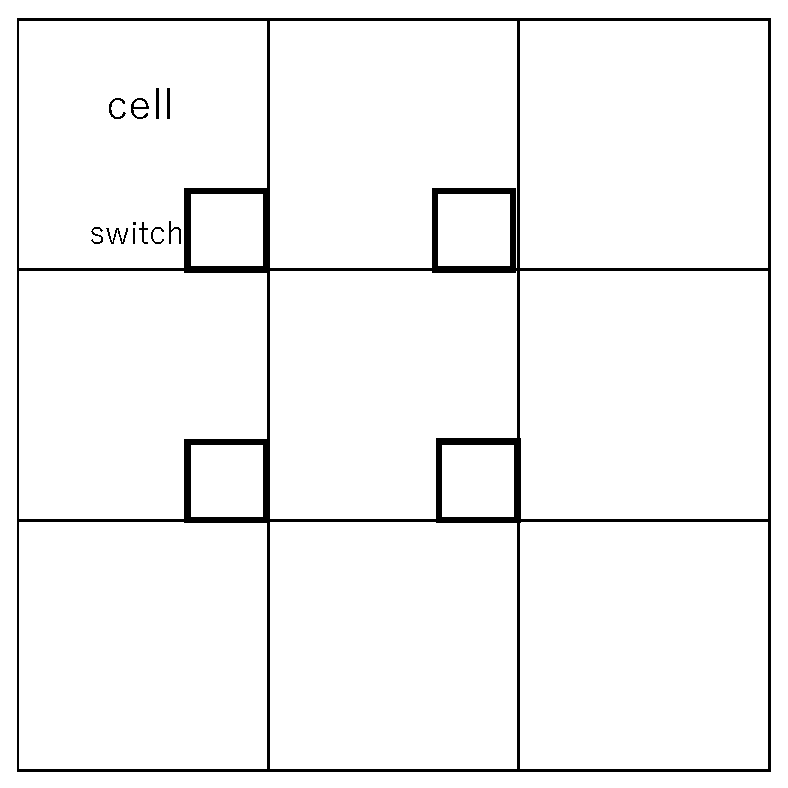
\includegraphics[keepaspectratio,scale=0.3]{fig/4/case1.eps}
\label{fig:all_switch_1}}
\subfigure[状態2]{
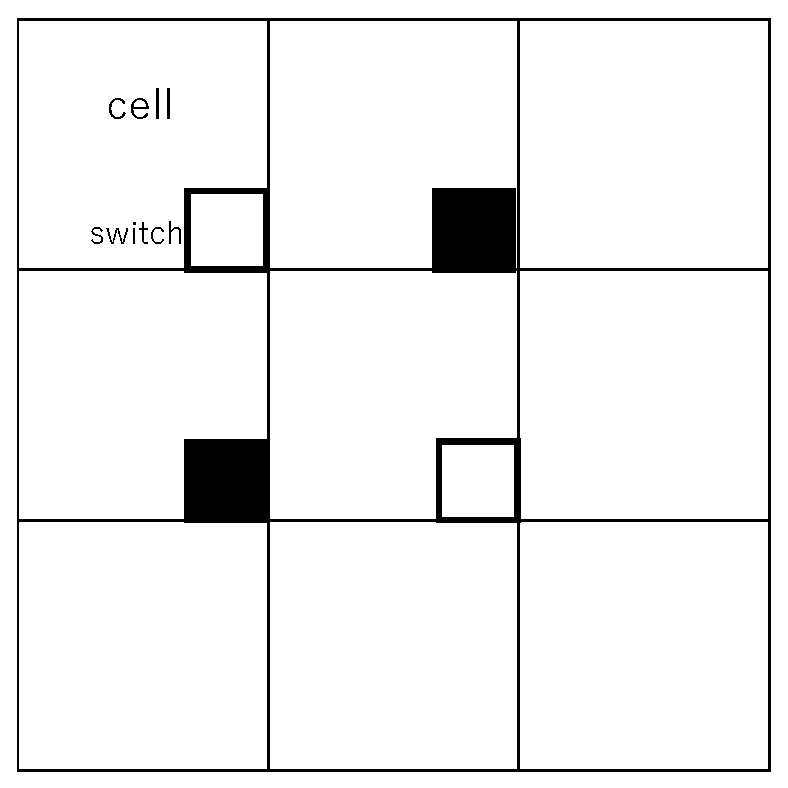
\includegraphics[keepaspectratio,scale=0.3]{fig/4/case2.eps}
\label{fig:all_switch_2}}
\subfigure[状態3]{
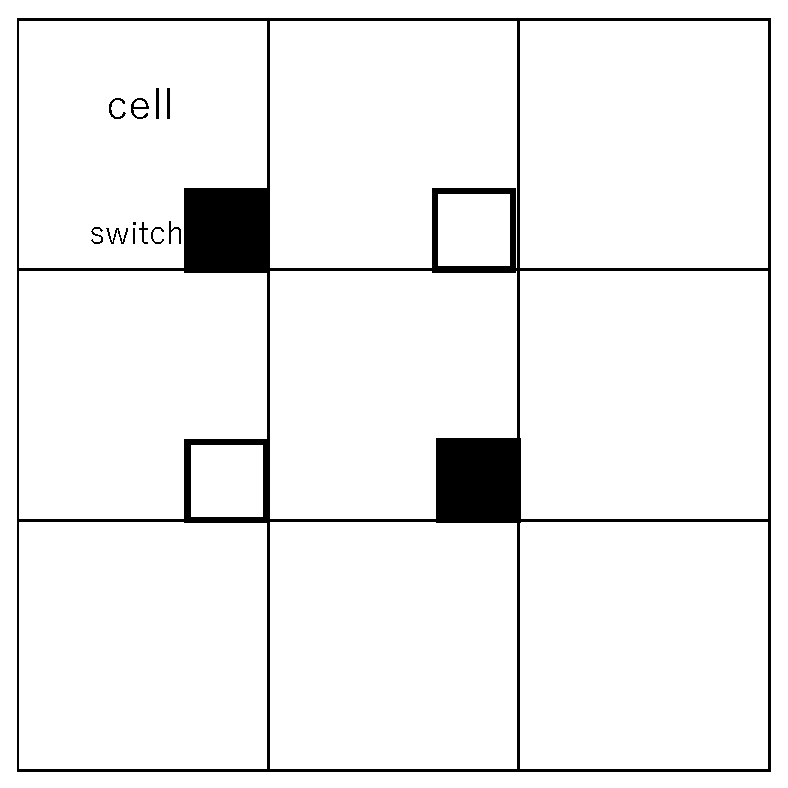
\includegraphics[keepaspectratio,scale=0.3]{fig/4/case3.eps}
\label{fig:all_switch_3}}\\
\subfigure[状態4]{
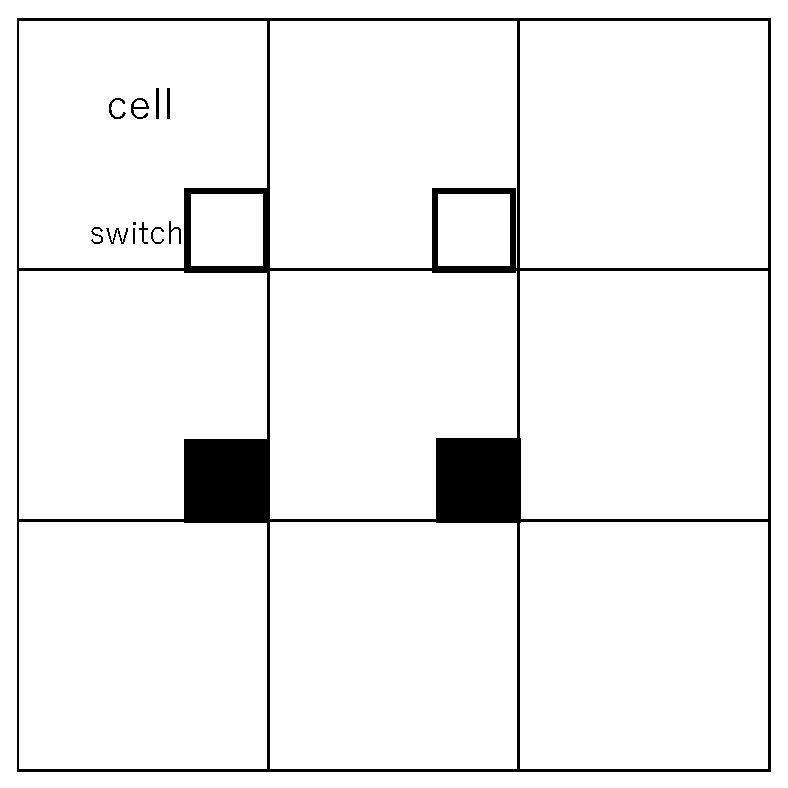
\includegraphics[keepaspectratio,scale=0.3]{fig/4/case4.eps}
\label{fig:all_switch_4}}
\subfigure[状態5]{
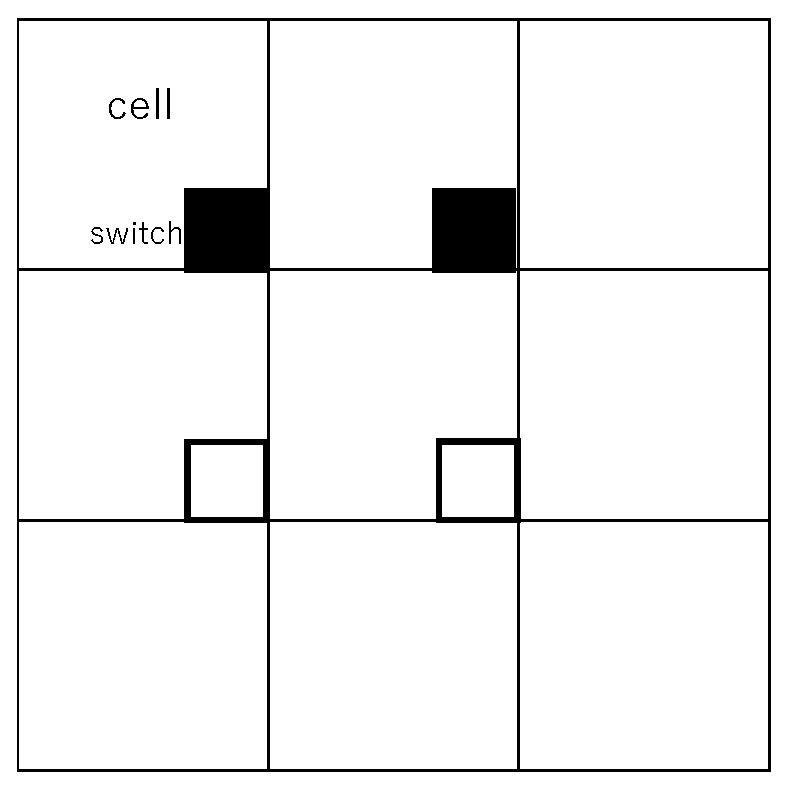
\includegraphics[keepaspectratio,scale=0.3]{fig/4/case5.eps}
\label{fig:all_switch_5}}
\subfigure[状態6]{
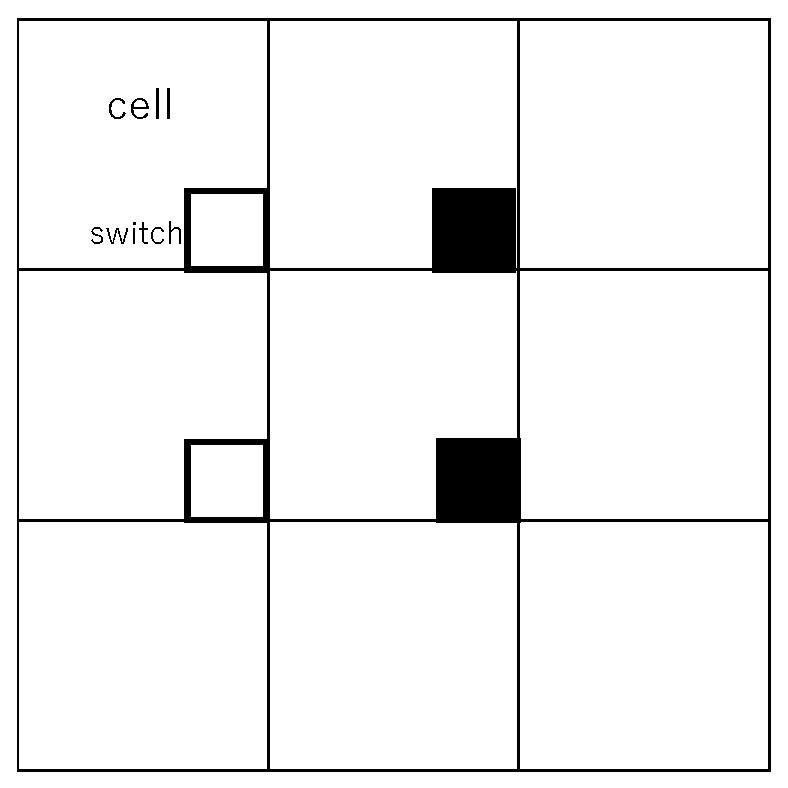
\includegraphics[keepaspectratio,scale=0.3]{fig/4/case6.eps}
\label{fig:all_switch_6}}\\
\subfigure[状態7]{
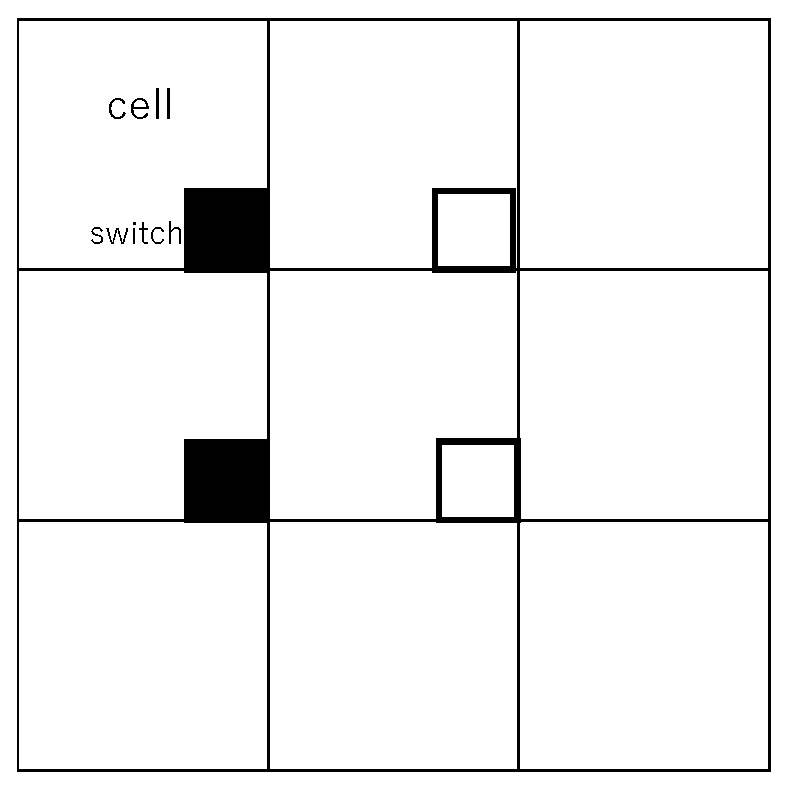
\includegraphics[keepaspectratio,scale=0.3]{fig/4/case7.eps}
\label{fig:all_switch_7}}
\subfigure[状態8]{
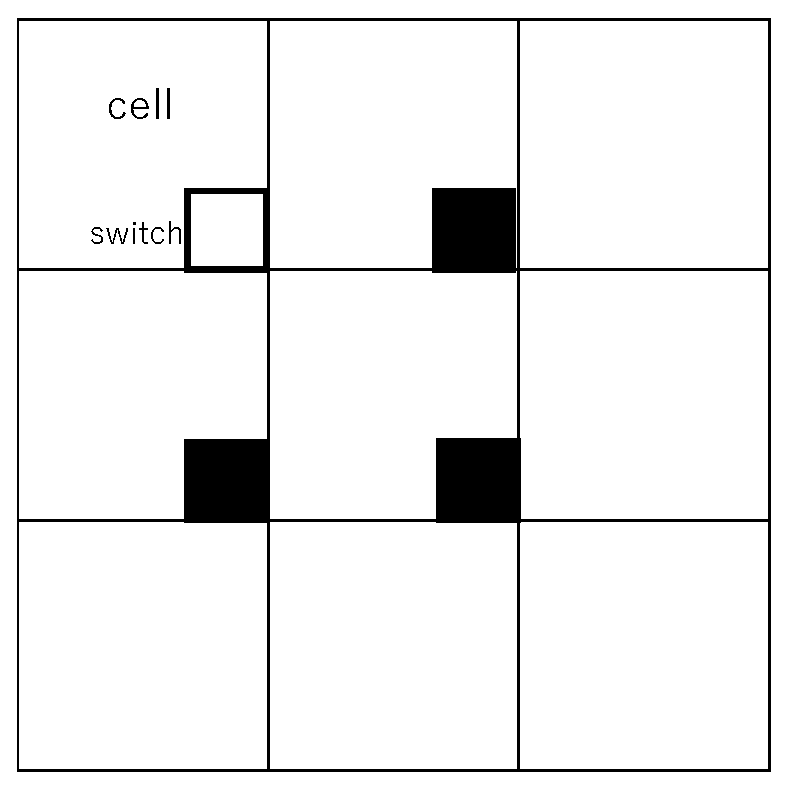
\includegraphics[keepaspectratio,scale=0.3]{fig/4/case8.eps}
\label{fig:all_switch_8}}
\subfigure[状態9]{
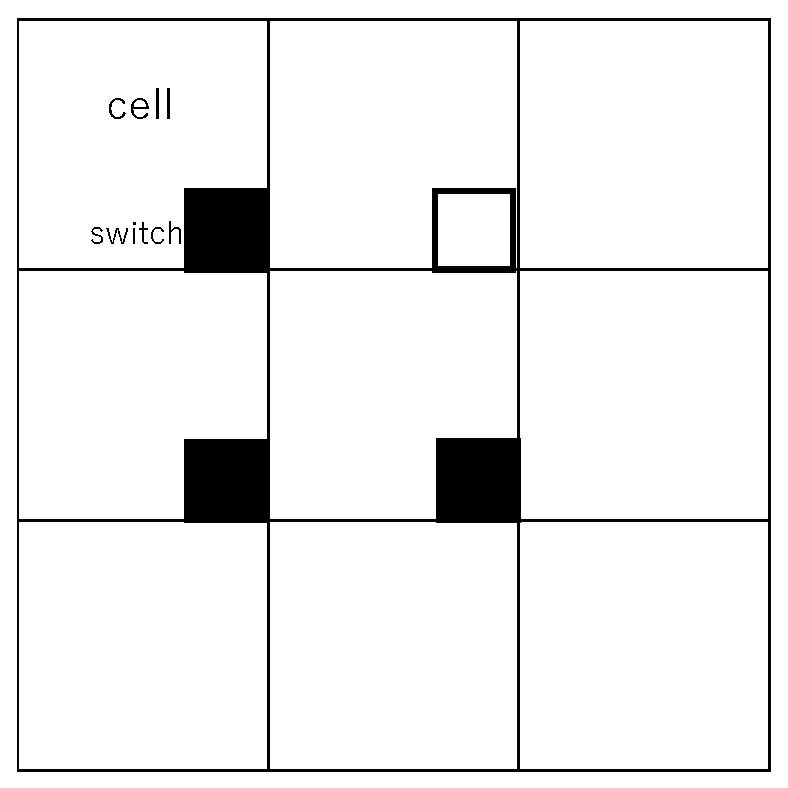
\includegraphics[keepaspectratio,scale=0.3]{fig/4/case9.eps}
\label{fig:all_switch_9}}\\
\subfigure[状態10]{
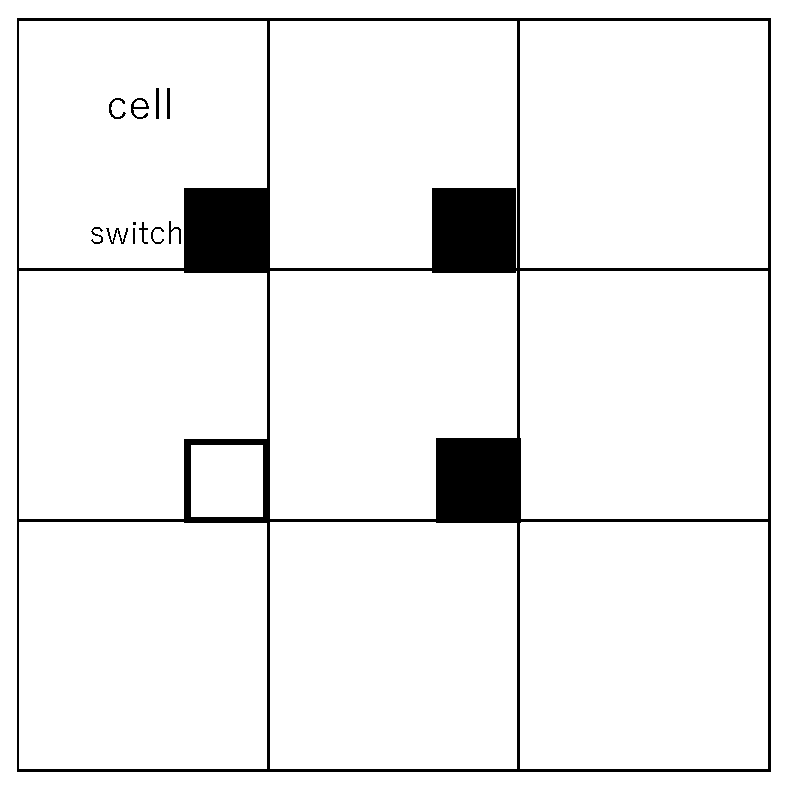
\includegraphics[keepaspectratio,scale=0.3]{fig/4/case10.eps}
\label{fig:all_switch_10}}
\subfigure[状態11]{
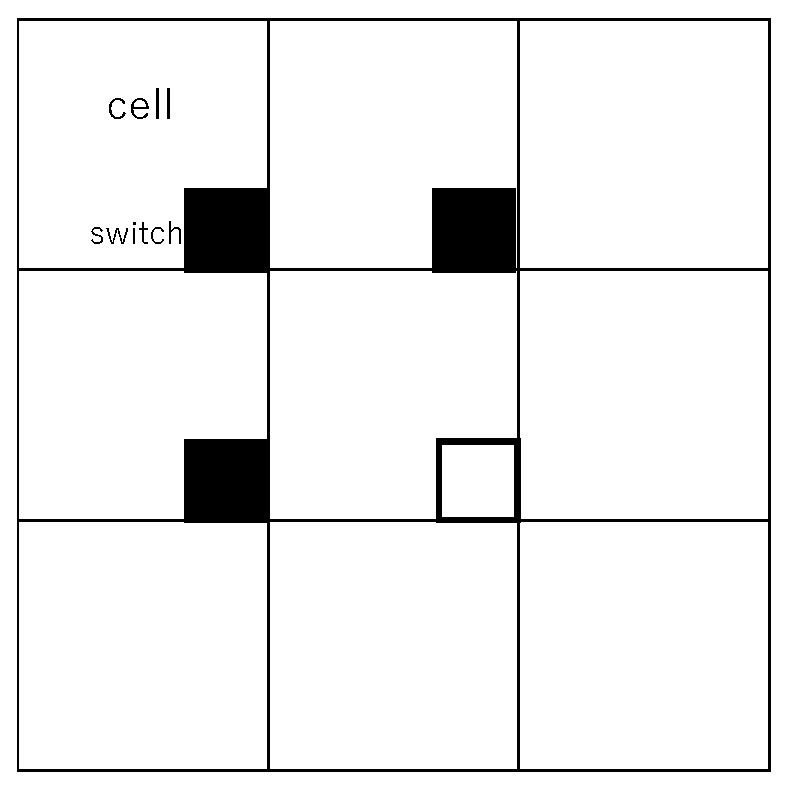
\includegraphics[keepaspectratio,scale=0.3]{fig/4/case11.eps}
\label{fig:all_switch_11}}
\subfigure[状態12]{
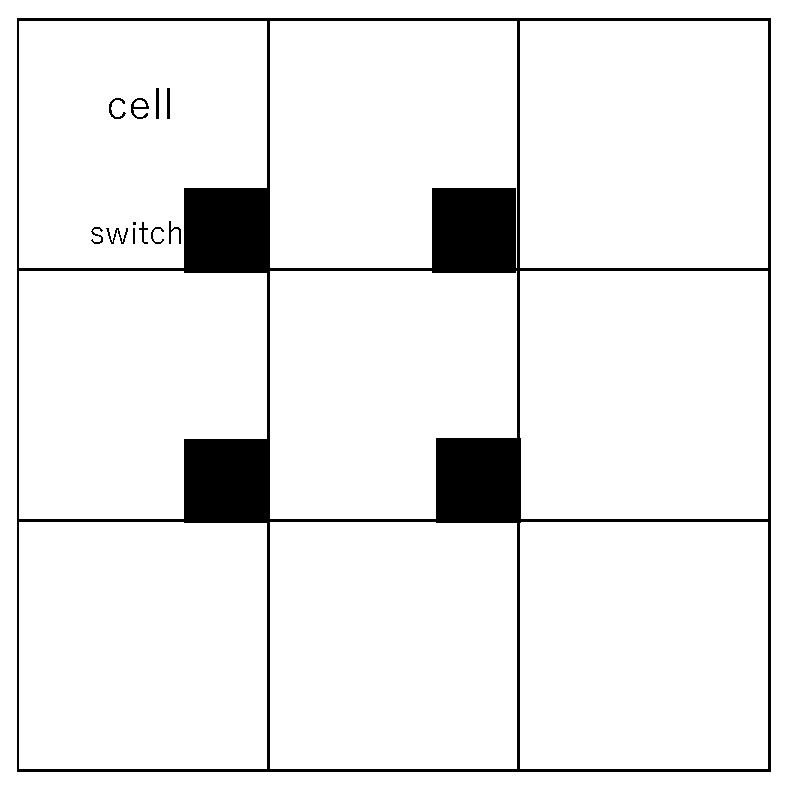
\includegraphics[keepaspectratio,scale=0.3]{fig/4/case12.eps}
\label{fig:all_switch_12}}\\
\caption{取りうる全スイッチの状態}
\label{fig:all_switch}
\end{center}
\end{figure}
\begin{figure}[t!]
\begin{center}
\subfigure[光Race Logic arrayへの光伝搬入力信号 1]{
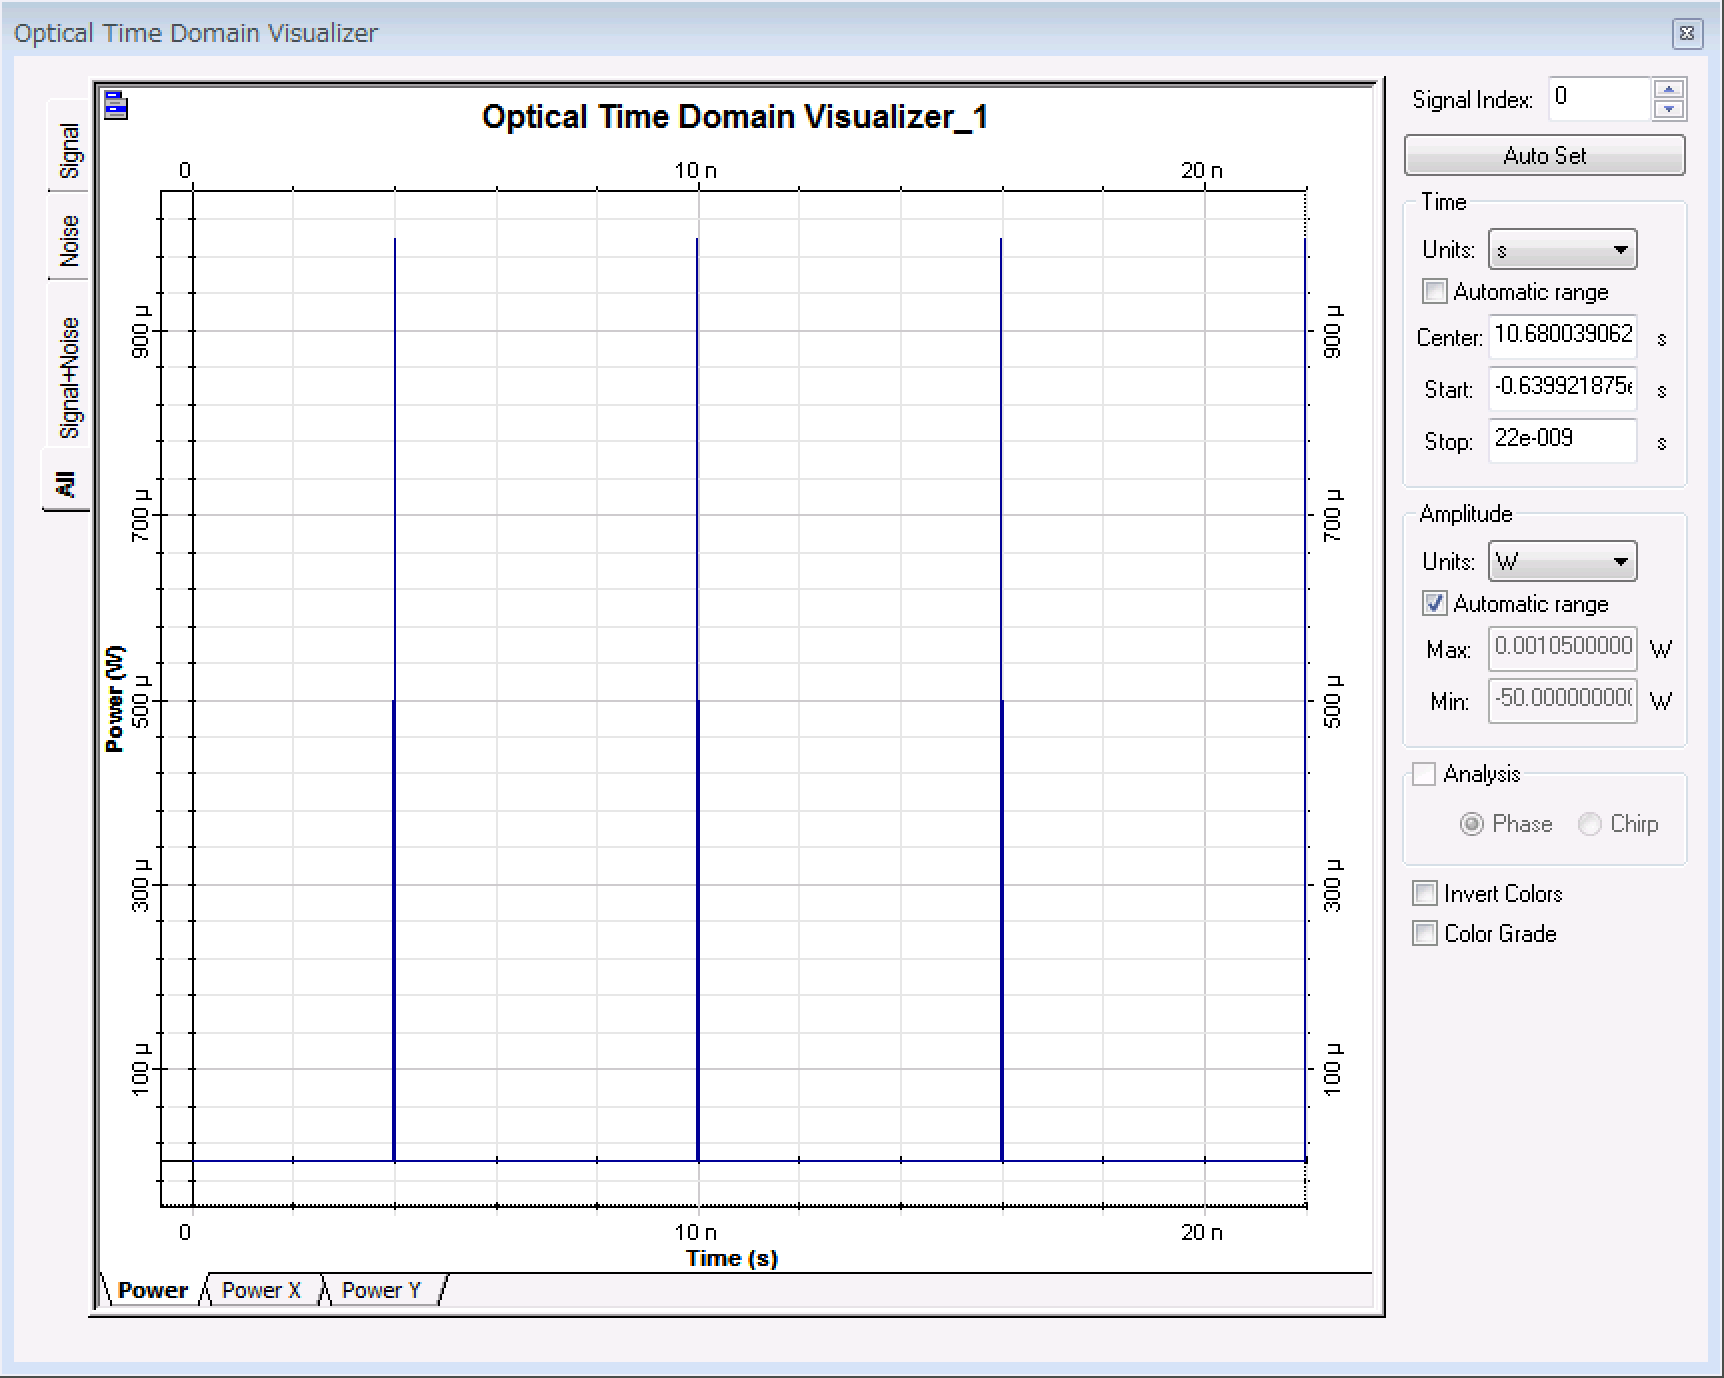
\includegraphics[keepaspectratio,scale=0.23]{fig/4/test_in1.png}
\label{fig:test_in1}}
\subfigure[光Race Logic arrayへの光伝搬出力信号 1]{
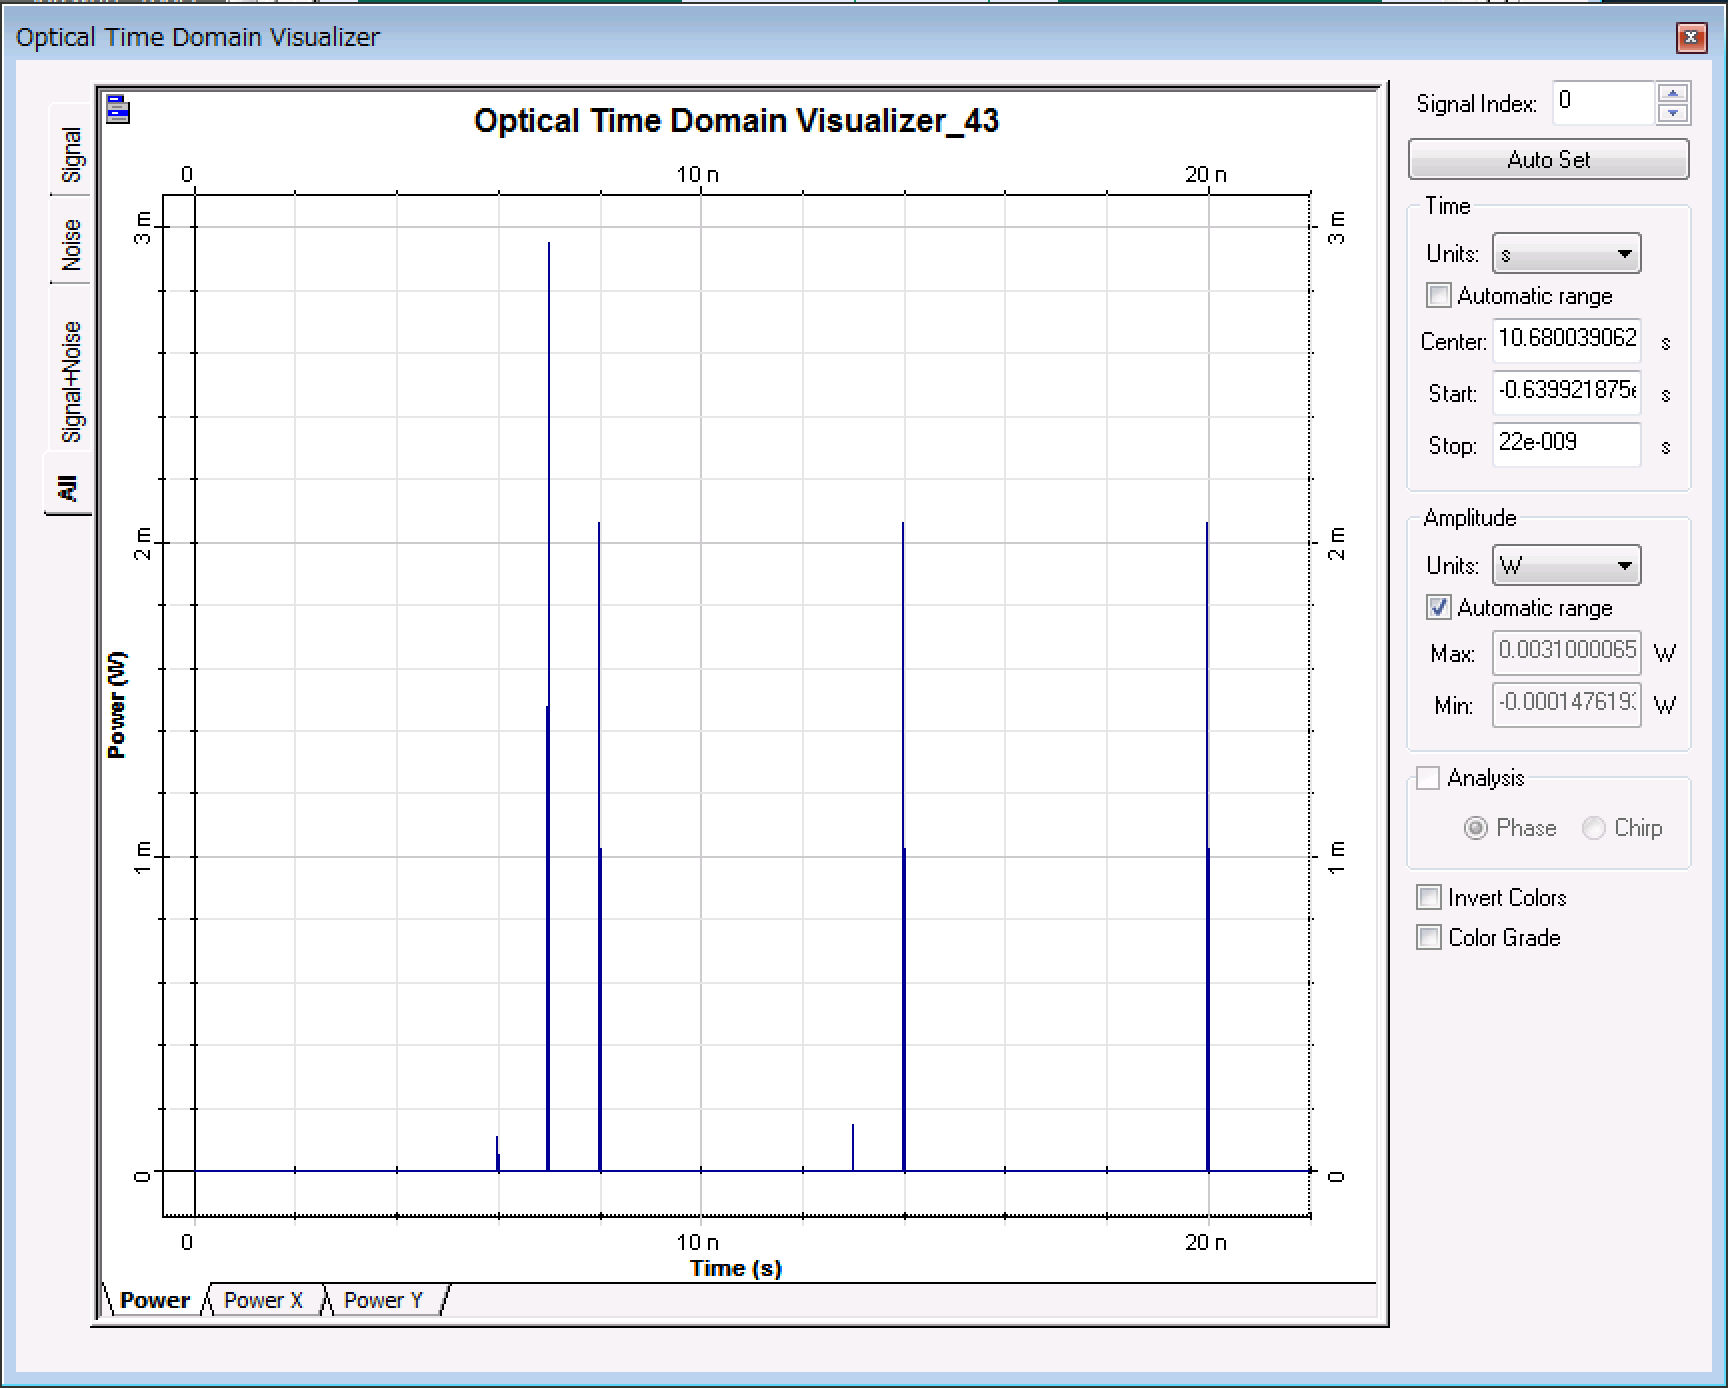
\includegraphics[keepaspectratio,scale=0.23]{fig/4/test_out1.png}
\label{fig:test_out1}}\\
\subfigure[光Race Logic arrayへの光伝搬入力信号 2]{
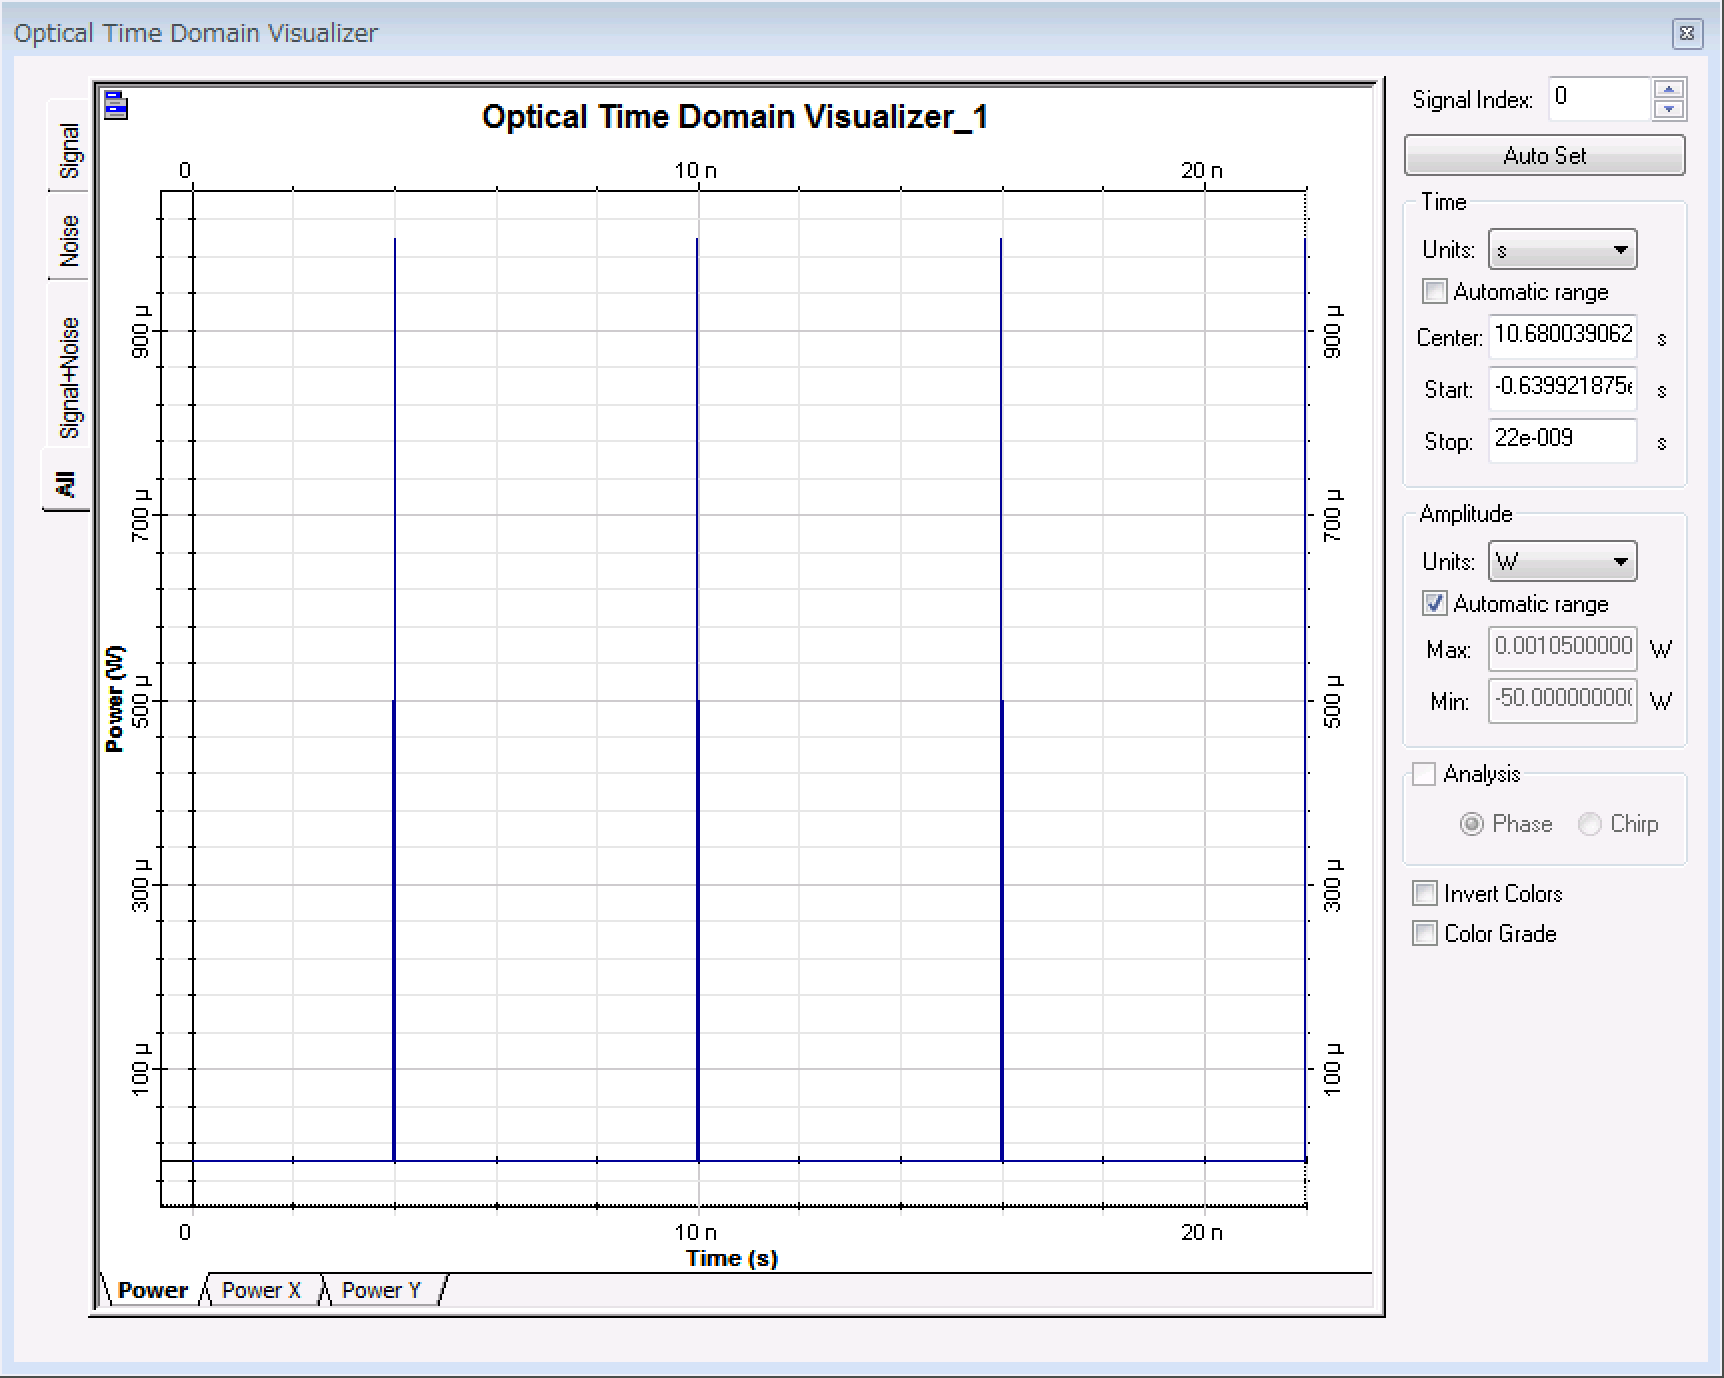
\includegraphics[keepaspectratio,scale=0.23]{fig/4/test_in2.png}
\label{fig:test_in2}}
\subfigure[光Race Logic arrayへの光伝搬出力信号 2]{
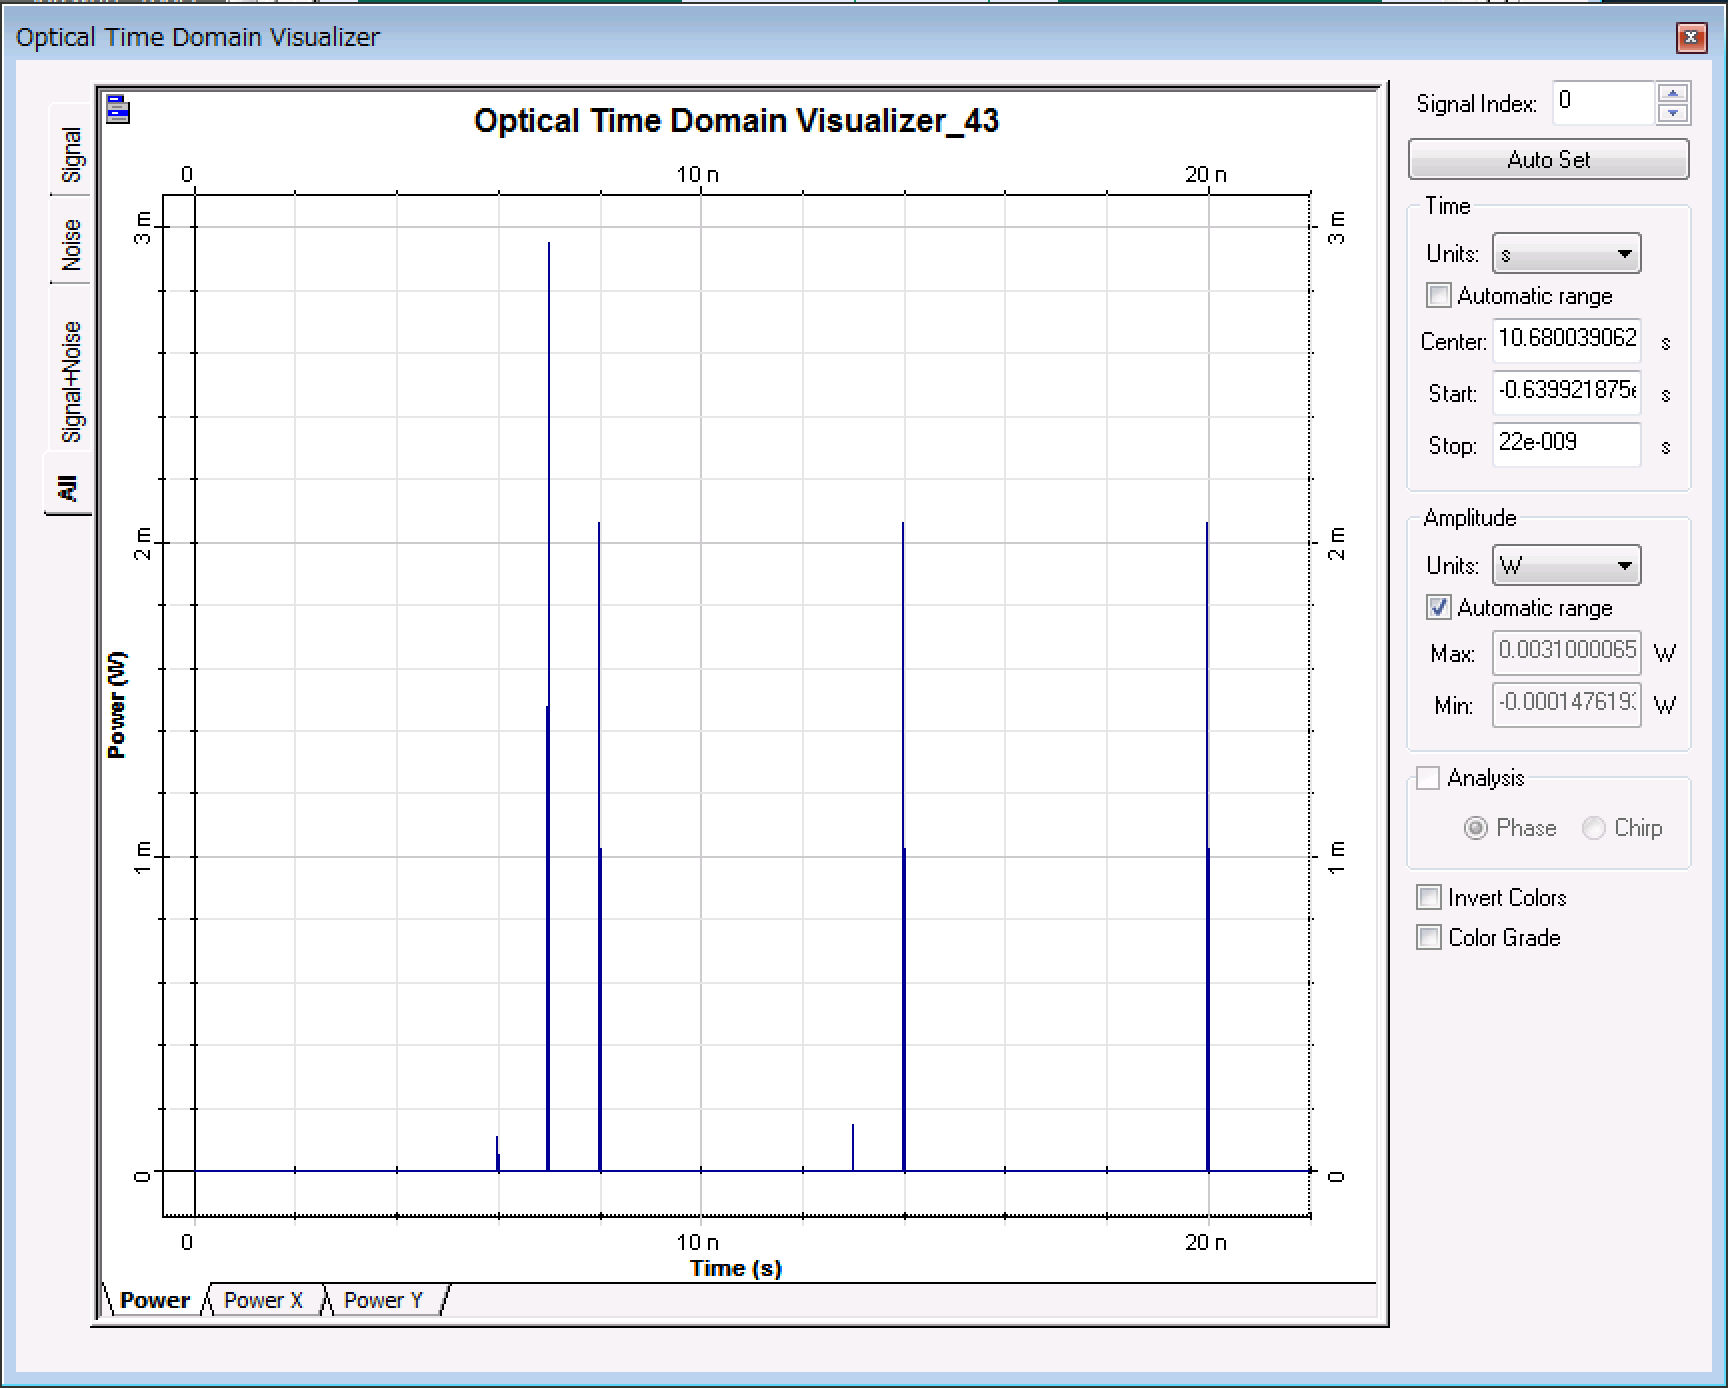
\includegraphics[keepaspectratio,scale=0.23]{fig/4/test_out2.png}
\label{fig:test_out2}}\\
\subfigure[光Race Logic arrayへの光伝搬入力信号 3]{
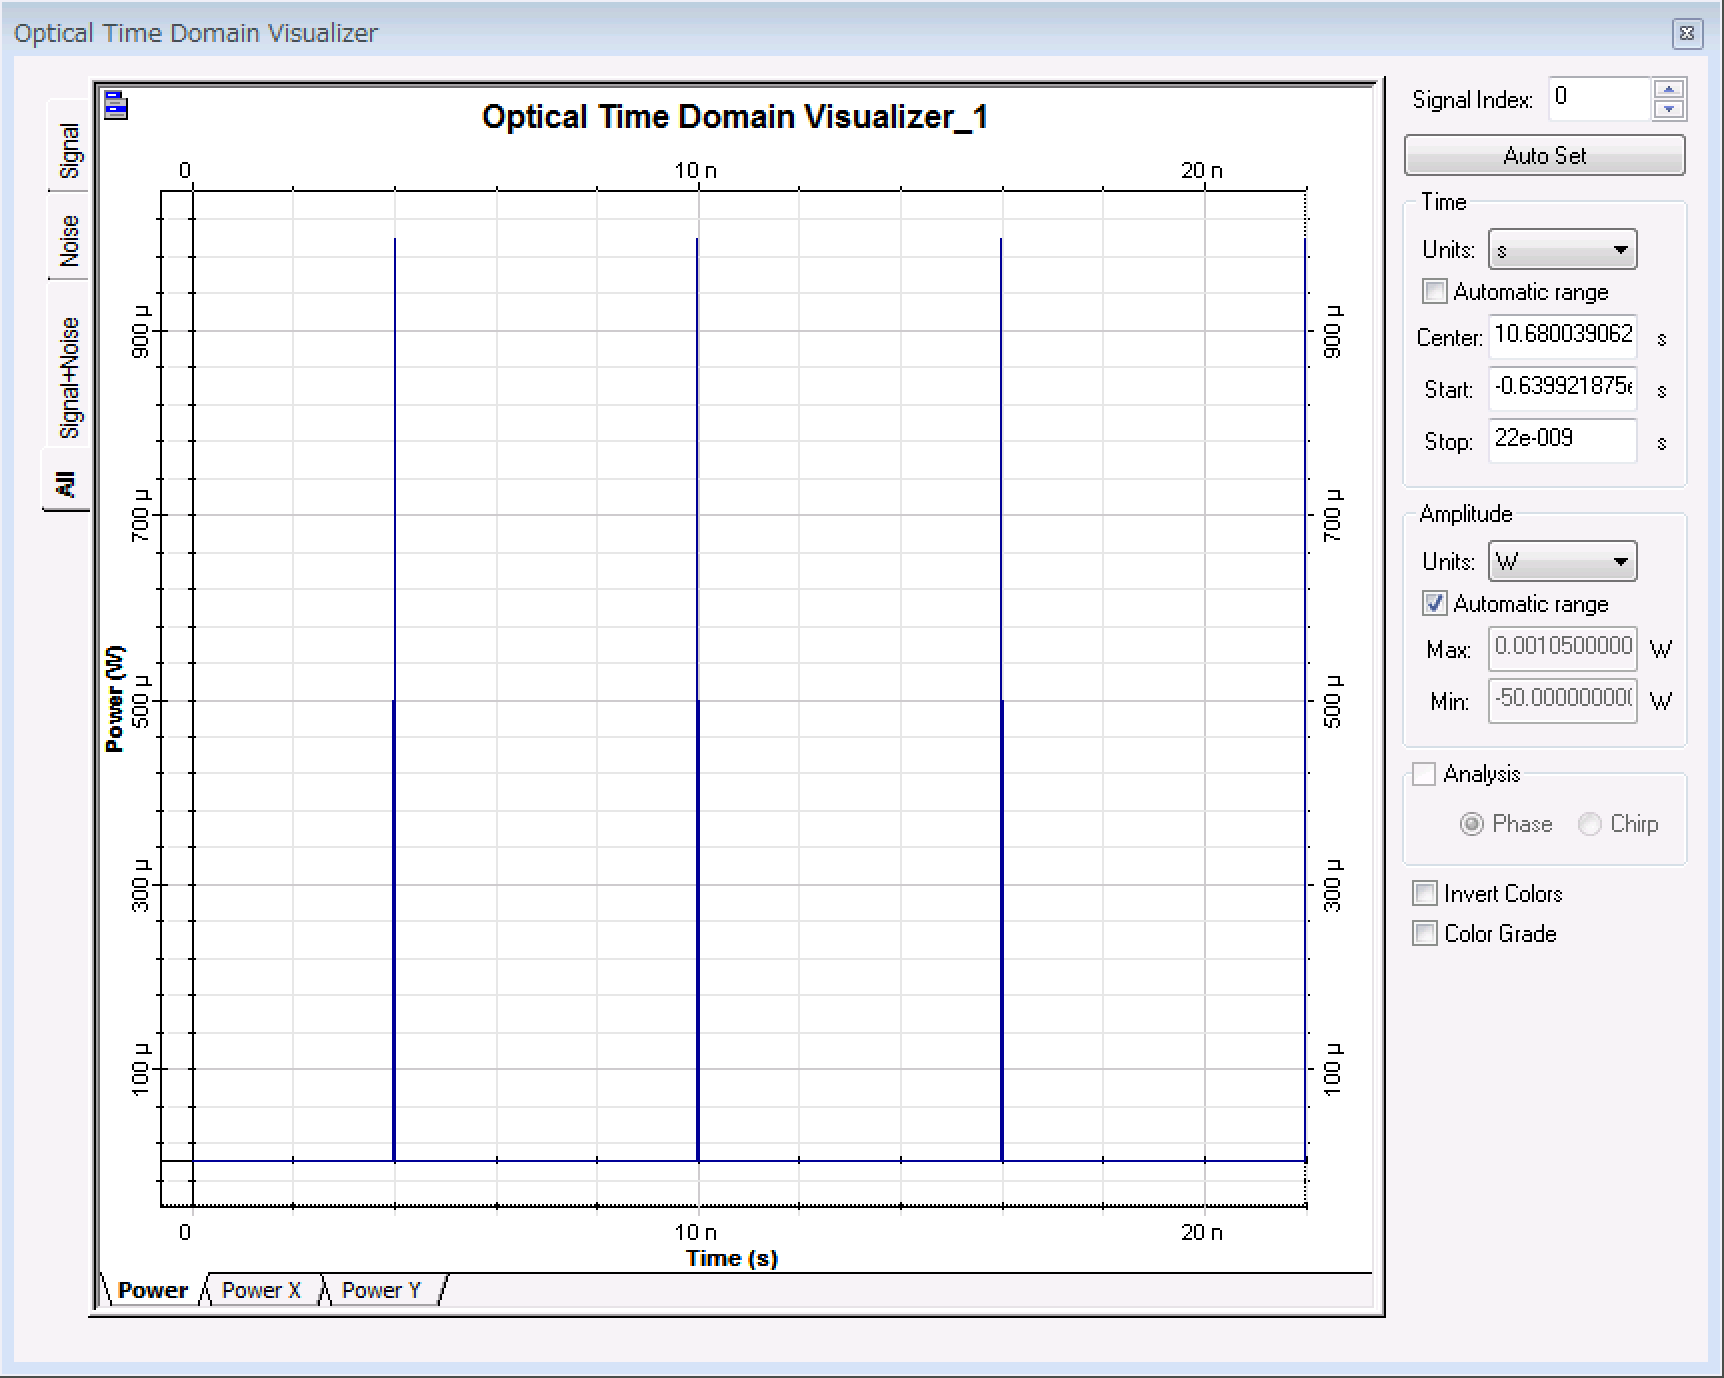
\includegraphics[keepaspectratio,scale=0.23]{fig/4/test_in3.png}
\label{fig:test_in3}}
\subfigure[光Race Logic arrayへの光伝搬出力信号 3]{
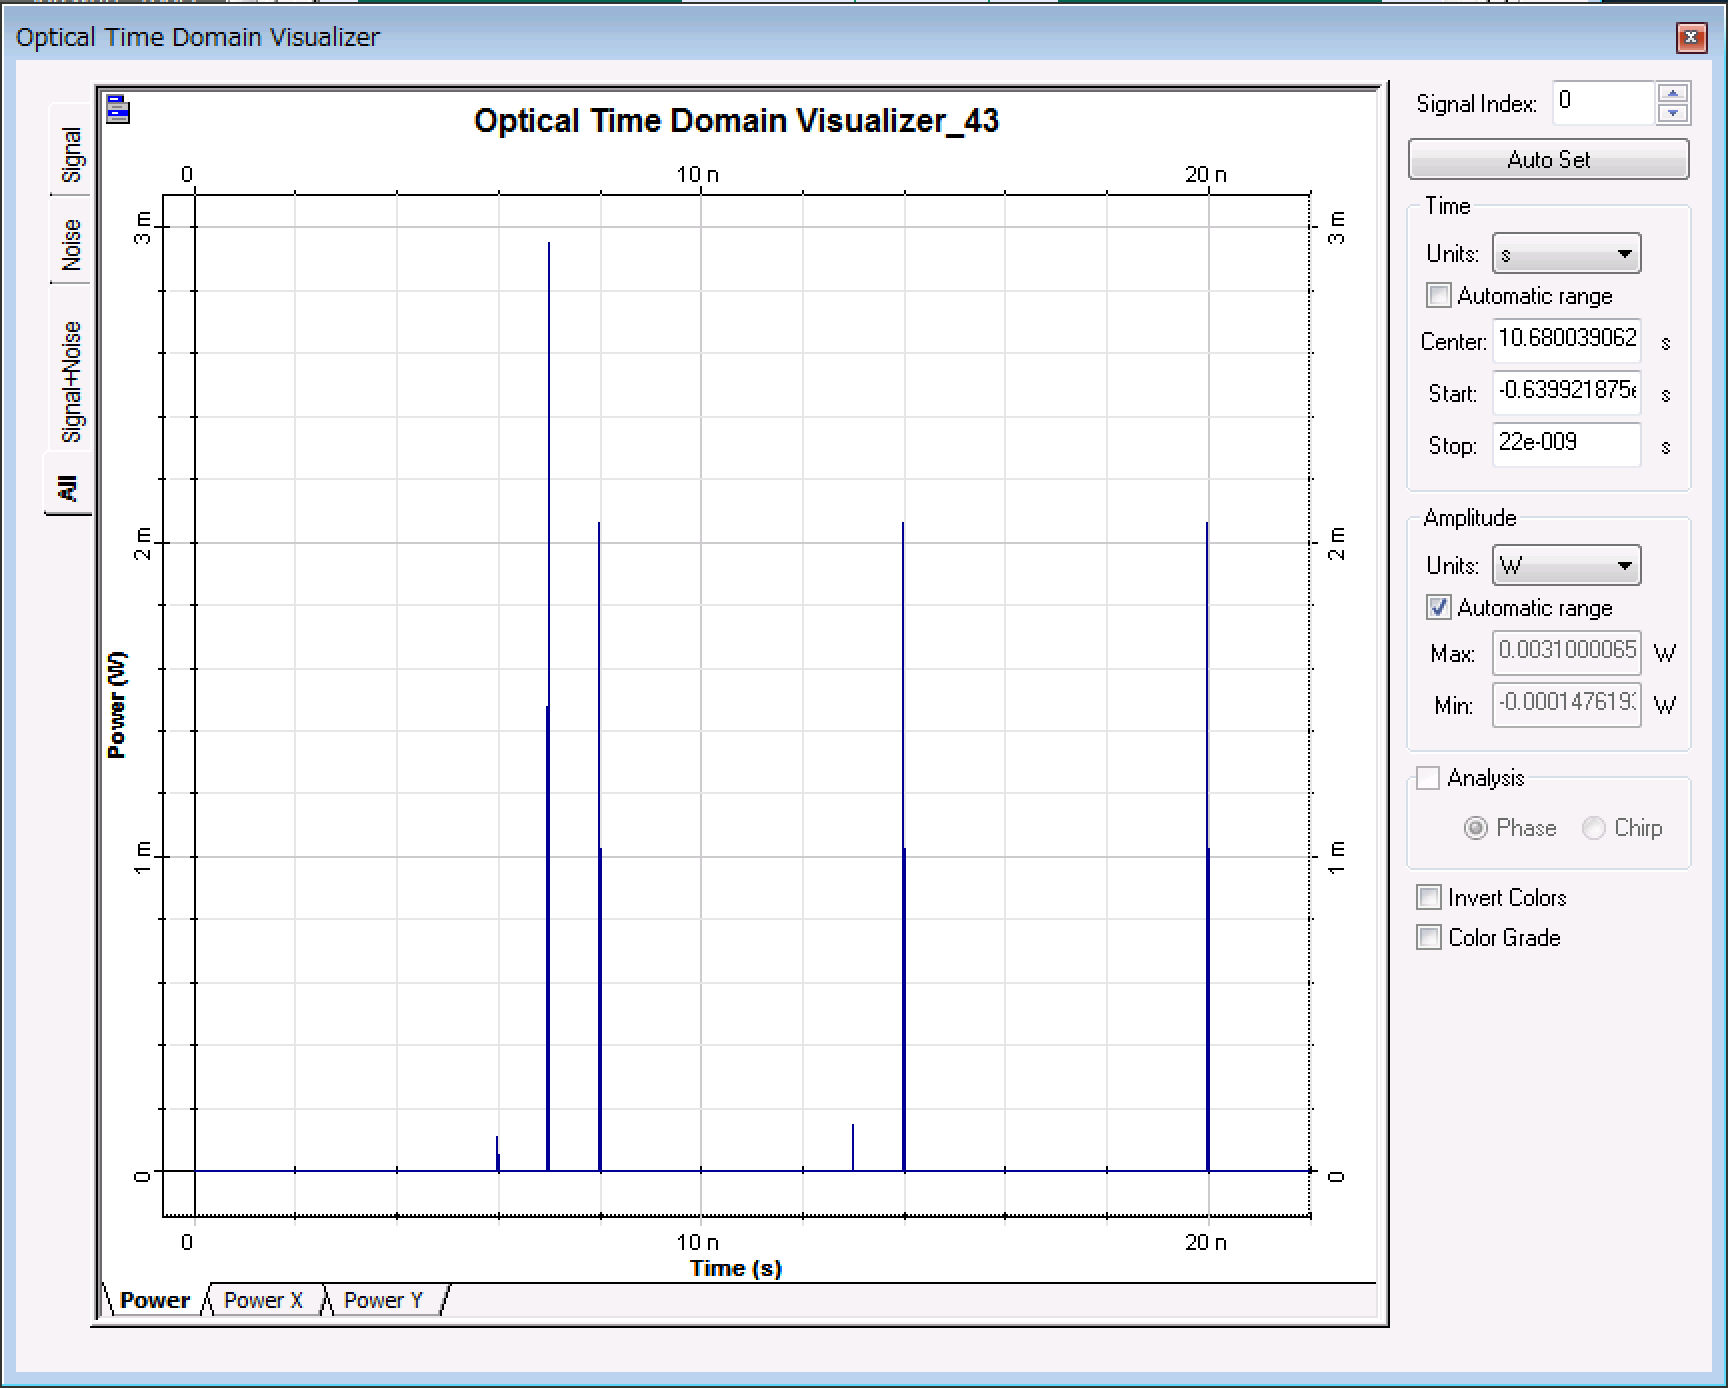
\includegraphics[keepaspectratio,scale=0.23]{fig/4/test_out3.png}
\label{fig:test_out3}}
\caption{Optisystemでの光伝搬入出力信号}
\label{fig:test}
\end{center}
\end{figure}

表\ref{test_timing}に,図\ref{fig:all_switch}のそれぞれの状態ごとの,
\begin{enumerate}
\item 最初の光伝搬出力信号の伝搬遅延時間の想定値
\item シミュレータ上の回路のスイッチがその状態を取る区間
\item 結果から読み取った最初の光伝搬出力信号の伝搬遅延時間
\end{enumerate}
を示す.
\begin{table}[t!]
\begin{center}
\caption{配列長N=2の光Race Logic arrayの動作検証結果}
\begin{tabular}{|c|c|c|c|} \hline
&1&2&3\\ \hline \hline
状態1&$2ns$&図\ref{fig:test_in1},\ref{fig:test_out1}の$ns〜ns区間$&$2ns$\\ \hline
状態2&$2ns$&図\ref{fig:test_in1},\ref{fig:test_out1}の$ns〜ns区間$&$2ns$\\ \hline
状態3&$3ns$&図\ref{fig:test_in1},\ref{fig:test_out1}の$ns〜ns区間$&$3ns$\\ \hline
状態4&$3ns$&図\ref{fig:test_in1},\ref{fig:test_out1}の$ns〜ns区間$&$3ns$\\ \hline
状態5&$3ns$&図\ref{fig:test_in2},\ref{fig:test_out2}の$ns〜ns区間$&$3ns$\\ \hline
状態6&$3ns$&図\ref{fig:test_in2},\ref{fig:test_out2}の$ns〜ns区間$&$3ns$\\ \hline
状態7&$3ns$&図\ref{fig:test_in2},\ref{fig:test_out2}の$ns〜ns区間$&$3ns$\\ \hline
状態8&$3ns$&図\ref{fig:test_in2},\ref{fig:test_out2}の$ns〜ns区間$&$3ns$\\ \hline
状態9&$3ns$&図\ref{fig:test_in3},\ref{fig:test_out3}の$ns〜ns区間$&$3ns$\\ \hline
状態10&$3ns$&図\ref{fig:test_in3},\ref{fig:test_out3}の$ns〜ns区間$&$3ns$\\ \hline
状態11&$3ns$&図\ref{fig:test_in3},\ref{fig:test_out3}の$ns〜ns区間$&$3ns$\\ \hline
状態12&$4ns$&図\ref{fig:test_in3},\ref{fig:test_out3}の$ns〜ns区間$&$4ns$\\ \hline
\end{tabular}
\label{test_timing}
\end{center}
\end{table}

この機能検証結果から,光Race Logic arrayが
想定した動作をしていることが確認できた.

\section{評価}
本節では,提案した光Race Logic arrayが
一組の配列のアラインメントを求める(以後,これを一計算と呼称する)ために必要な
遅延時間や面積及び消費電力が
配列長Nによってどう変化するかを見積るために
各項目を算出するモデル式を構築し,評価を行う.

\subsection{遅延時間}
光Race Logic arrayに光伝搬信号が入射されてからarray内を伝搬し,
最初に出力された信号が受光器で検出されるまでの遅延時間を考える.
配列長Nの光Race logic arrayにおいて,最初に光伝搬信号が出力されるまでの回路遅延時間は
配列の組み合わせによって異なる.
二つの配列が完全に不一致の場合,最初に光伝搬信号が出力されるまでの回路遅延時間は
最長となる.
今回はこのワーストケースの遅延時間をモデル化した.

図\ref{fig:proposalcell}の構造より構築した遅延時間$T$のモデル式を式\ref{eq:latency}に示す.
\begin{eqnarray}
&&T = T_{wire}+2N \times T_{cell-pass}+T_{pd} \nonumber \\
&&T_{cell-pass} = T_{cell-wire}+T_{coupler}+T_{amp}+T_{splitter}+T_{switch-pass}
\label{eq:latency}
\end{eqnarray}

$T_{wire}はセル間の配線遅延時間,T_{cell-pass}は一つのセルを通過する遅延時間,T_{pd}は受光器の応答時間である.$
$T_{cell-pass}の内訳はT_{cell-wire}がセル内部の配線遅延,$
$T_{coupler}・T_{splitter}がそれぞれ光結合器・光分配器の遅延時間,$
$T_{amp}がアンプの遅延時間,T_{switch-pass}が光スイッチ遅延時間である.$
$T_{wire}とT_{cell-pass}が光伝搬入力信号が$光Race Logic array$を伝搬するために必要な時間,$
$T_{pd}が受光器が光出力信号を検出するまでに必要な時間である.$
式\ref{eq:latency}に示す通り,遅延時間は
配列長Nに線形にスケーリングする.

光伝搬信号は光デバイス内部を光速で通過するため,光デバイス内の遅延時間は素子のゲート長に依存する.
今回は,ナノフォトニック・デバイスのゲート長が100,10,1$\mu m$の場合の
光Race Logic arrayの遅延時間を示す.
なお,配線遅延に関しては今回は無視している.
図\ref{fig:nanolatency}の縦軸は遅延時間,横軸は配列長Nである.
図\ref{fig:nanolatency}より,ナノフォトニック・デバイスのゲート長が小さいほど
遅延時間が小さくなることが読み取れる.
\begin{figure}[t!]
\begin{center}
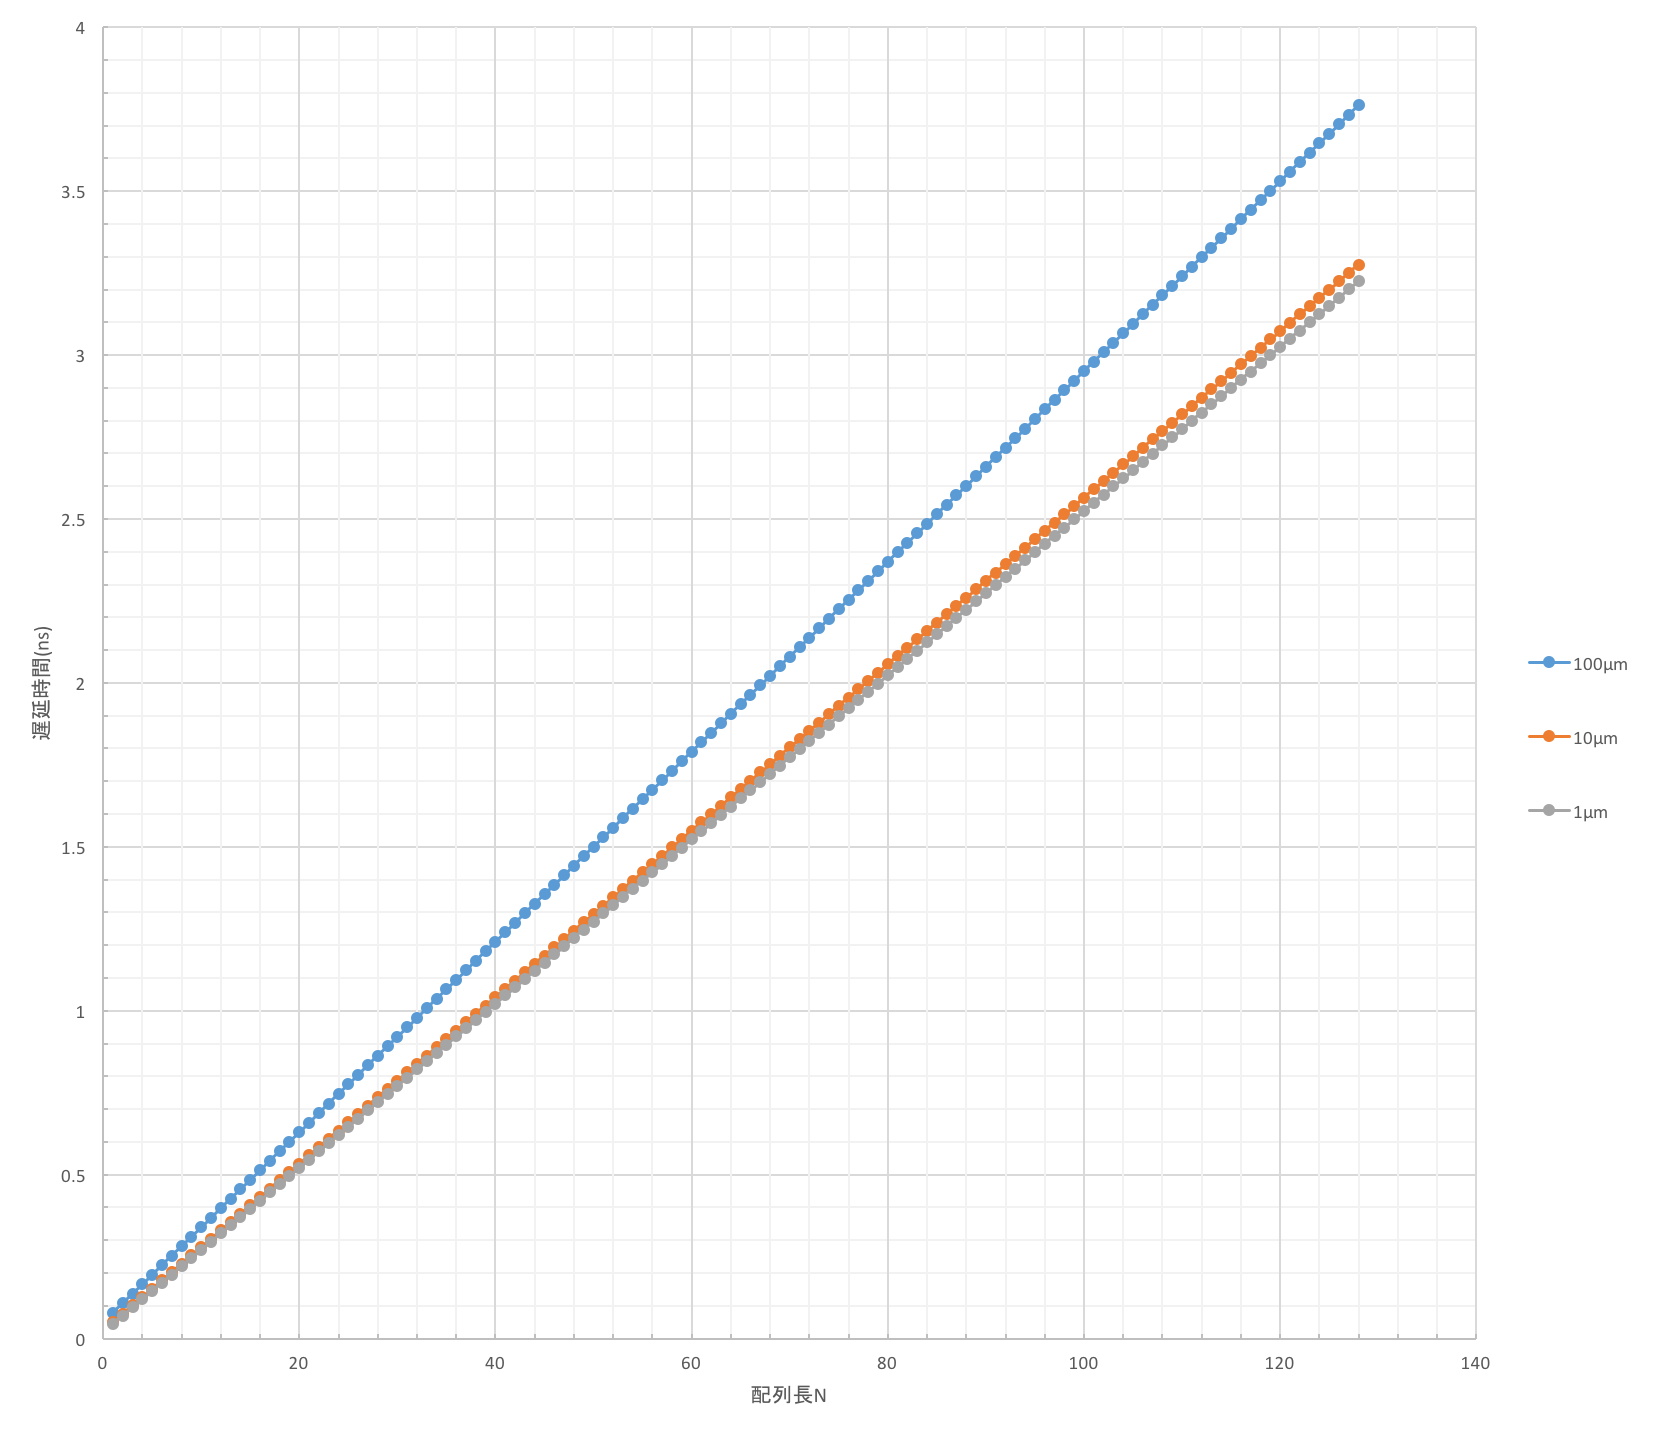
\includegraphics[keepaspectratio,scale=0.5]{fig/4/nanolatency.png}
\caption{光Race Logic arrayの遅延時間}
\label{fig:nanolatency}
\end{center}
\end{figure}

\subsection{面積}
提案したセルの構成(図\ref{fig:proposalcell})より,
セル一つの面積$A_{cell}$を表すモデル式は式\ref{eq:cellArea}と書ける.
\begin{equation}
A_{cell} = A_{cell-wire}+A_{coupler}+A_{amp}+A_{splitter}+A_{switch}+2A_{delay}
\label{eq:cellArea}
\end{equation}

$A_{cell-wire}はセル内部の配線面積,A_{amp}がアンプの面積,$
$A_{coupler}・A_{splitter}はそれぞれ光結合器・光分配器の遅延時間,$
$A_{switch}が光スイッチの面積,A_{delay}は光遅延素子の面積である.$
このセルを基準セルとする.

セルを並べてarrayを構成した時に,図\ref{fig:N=2}に示すように,
外周のセルはこの基準セルとは違う構成となる.
この差異に留意しながら,配列長Nの光Race logic arrayの面積$A$をモデル化した.
モデル式を式\ref{eq:Area}に示す.
\begin{equation}
A = A_{wire}+N^2 \times A_{cell} + 2N \times (A_{delay}+A_{amp}) +A{ls}+A_{pd}
\label{eq:Area}
\end{equation}

$A_{wire}はセル間の配線面積,A{ls}は光源の面積,A_{pd}は受光器の面積である.$
式\ref{eq:Area}が示すように,面積は
配列長Nの2乗にスケーリングする.

ナノフォトニック・デバイスのゲート長が100,10,1$\mu m$の場合の
光Race Logic arrayの面積を示す.
なお,配線面積に関しては今回は無視している.
図\ref{fig:nanoArea}の縦軸は光Race Logic arrayの面積,横軸は配列長Nである.
\begin{figure}[t!]
\begin{center}
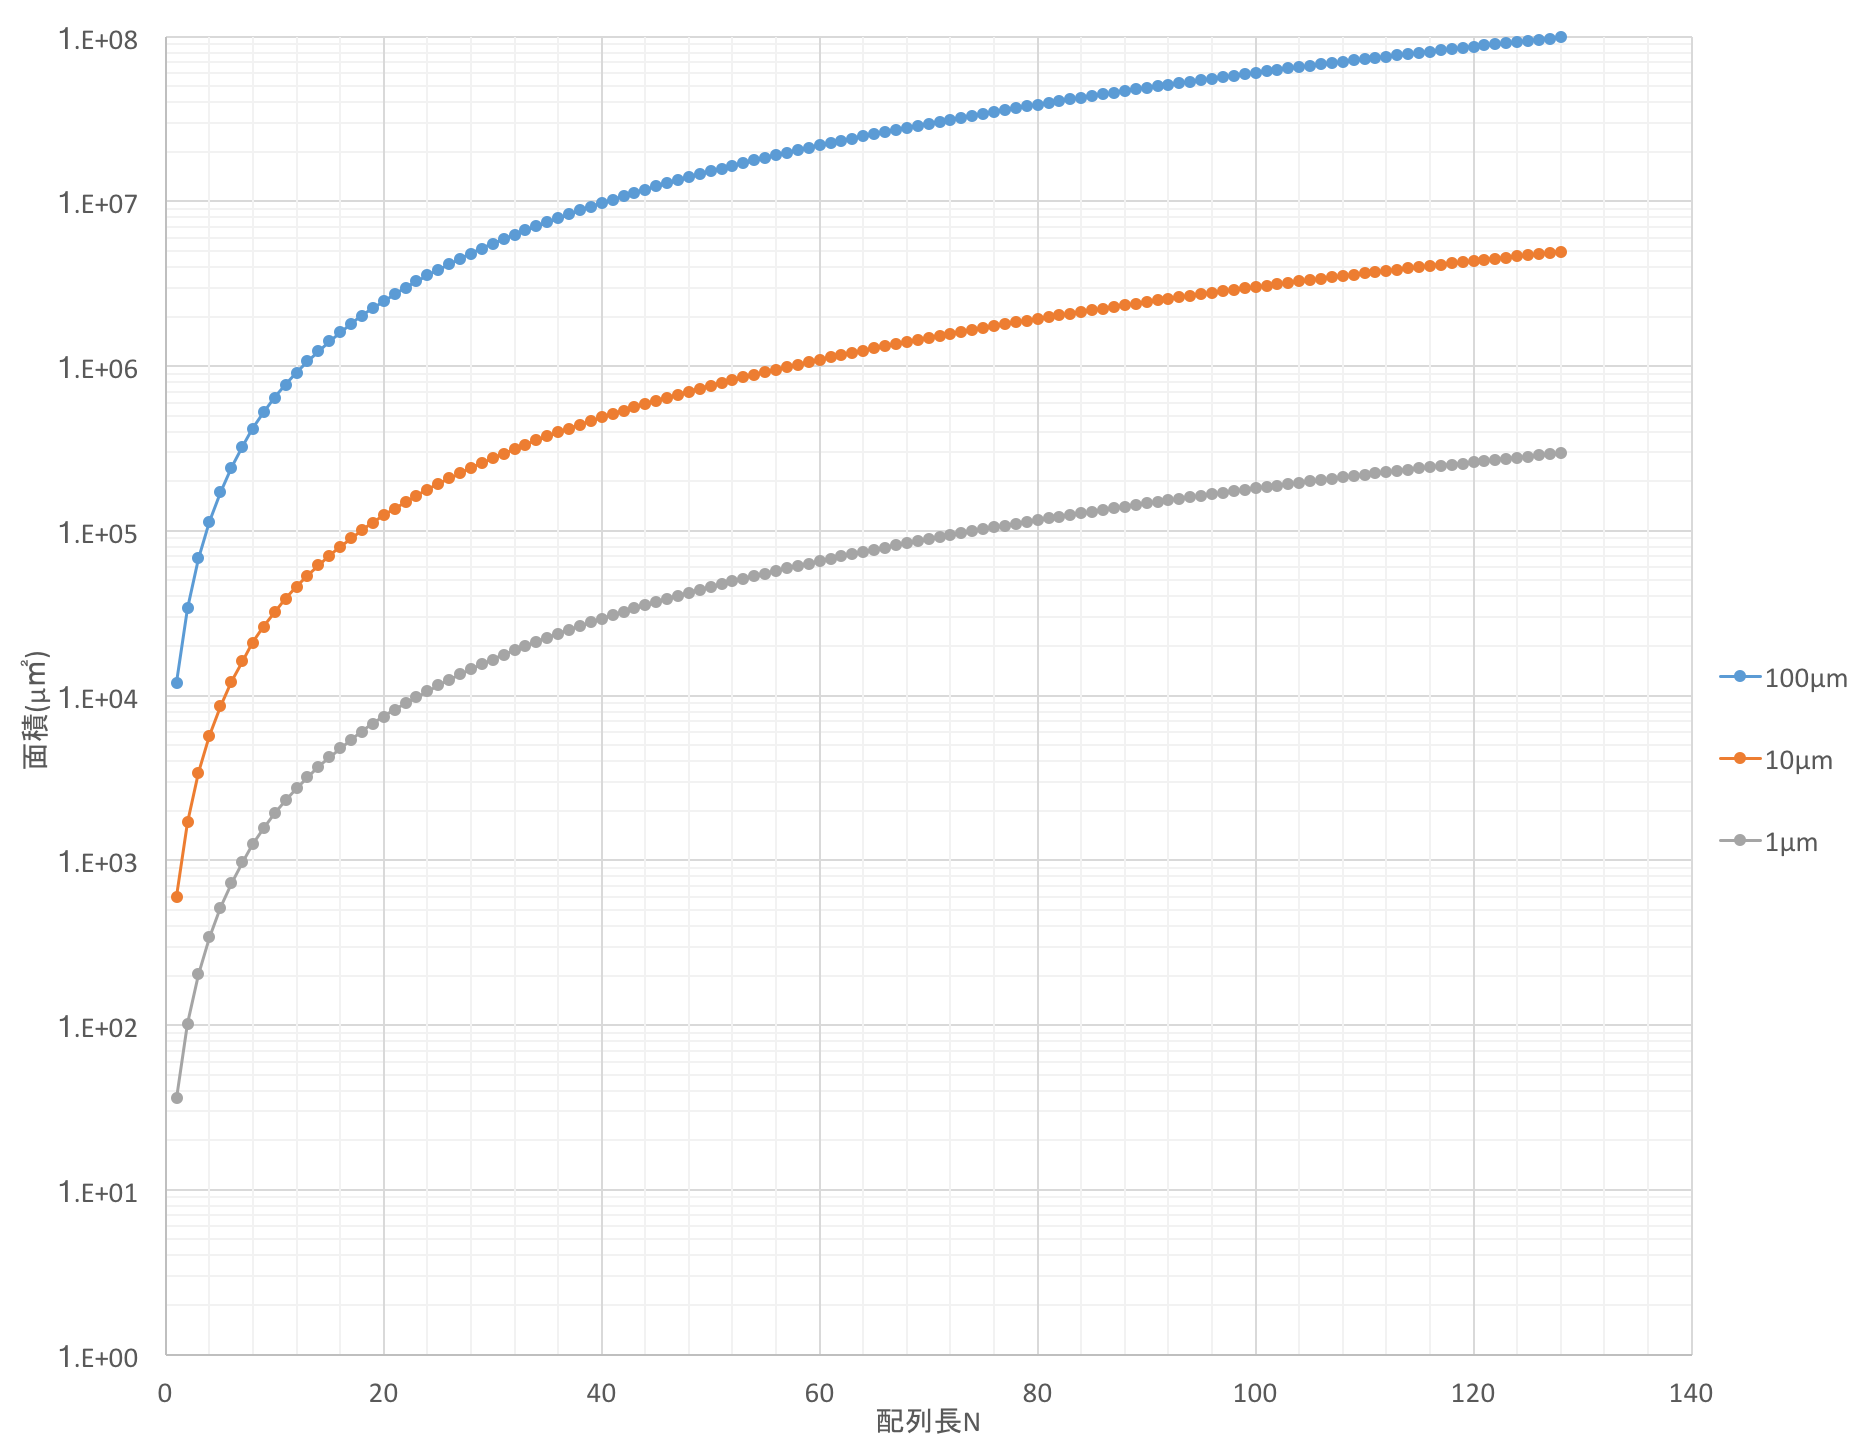
\includegraphics[keepaspectratio,scale=0.5]{fig/4/nanoArea.png}
\caption{光Race Logic arrayの面積}
\label{fig:nanoArea}
\end{center}
\end{figure}

\subsection{消費電力}
ここで本提案の光Race Logic arrayでの消費電力について考える.
この回路での消費電力は,式\ref{eq:power}に示すように
$光源の消費電力P_{ls}$,$アンプP_{amp}$の消費電力の二つのみで考えることができる.
\begin{equation}
P=P_{ls}+P_{amp}
\label{eq:power}
\end{equation}

$P$の値は,光Race Logic arrayが機能を担保できる値に設定しなければならない.
そこで,光Race Logic arrayの機能担保について具体的に見ていく.

配列長Nの光Race Logic arrayのN行N列目のセルからの
光伝搬出力信号強度$P_{out\,N,N}$は
式\ref{eq:power_out}と表せる.
\begin{equation}
P_{out\,N,N}=Loss_{N,N}(P_{out\,(N-1),(N-1)}+P_{out\,(N-1),N}+P_{out\,N,(N-1)})
\label{eq:power_out}
\end{equation}

$N \geq 0,P_{out\,-1,-1}=P_{ls},P_{out\,-1,0}=0,P_{out\,0,-1}=0である.$
$Loss_{N,N}$はN行N列目のセルに光伝搬信号が入力されてから出力される際のロスである.

$P_{out\,N,N}$の値は配列の組み合わせ,即ちスイッチの状態によって大きく変化する.
光Race Logic arrayからの光伝搬出力信号は受光器で検出されなければならない.
受光器の最小受光感度$P_{r}$を用いると,
$P_{out\,N,N}の最小値 \geq P_{r}となるようにP$の値を決定することが必要となる.

\subsubsection{ケーススタディ:配列長N=2の光Race logic arrayにおける消費電力}
ここで,図\ref{fig:loss}に示すように各素子における損失が一律で$\alpha$の場合において,
配列長N=2の光Race logic arrayにおける消費電力を考える.
\begin{figure}[t!]
\begin{center}
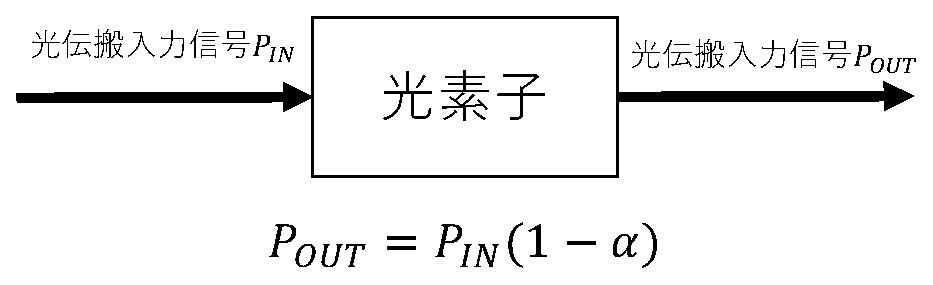
\includegraphics[keepaspectratio,scale=0.5]{fig/4/loss.eps}
\caption{光素子における損失例}
\label{fig:loss}
\end{center}
\end{figure}
この$\alpha$は0〜1の範囲の値を取る.
図\ref{fig:proposalcell}に示すセルにおいて,光信号を伝搬させる際に損失を与える素子は
光結合器,光分配器,光スイッチ,光遅延素子とする.
この4つの素子での損失を$\alpha$とし,その他の損失は考えない.
今回は回路規模が小さいので,各セルのアンプユニットでの
光伝搬信号強度の増幅は行わず,
光源の光出力信号強度を変えることによって$P_{out\,N,N}の最小値 \geq P_{r}となるように$する.
この光Race logic arrayの消費電力$PはP=P_{ls}$となる.

配列長N=2の光Race logic arrayの光スイッチは,
図\ref{fig:all_switch}に示す12通りのいずれかの状態を取る.
各状態での出力を以下に示す.
\begin{itemize}
\item 状態1(図\ref{fig:all_switch_1})の出力 $P_{out\,2,2}=P_{ls}\frac{(1-\alpha)^6}{3^2}$\\
\item 状態2(図\ref{fig:all_switch_2})の出力 $P_{out\,2,2}=P_{ls}\frac{(1-\alpha)^6}{3^2}$\\
\item 状態3(図\ref{fig:all_switch_3})の出力 $P_{out\,2,2}=P_{ls}\frac{2(1-\alpha)^7}{3^2}$\\
\item 状態4(図\ref{fig:all_switch_4})の出力 $P_{out\,2,2}=P_{ls}\frac{(1-\alpha)^7\bigl\{2(1-\alpha)+1\bigl\}}{3^2}$\\
\item 状態5(図\ref{fig:all_switch_5})の出力 $P_{out\,2,2}=P_{ls}\frac{(1-\alpha)^7\bigl\{\frac{2}{3}(1-\alpha)+1\bigl\}}{3^2}$\\
\item 状態6(図\ref{fig:all_switch_6})の出力 $P_{out\,2,2}=P_{ls}\frac{(1-\alpha)^7\bigl\{2(1-\alpha)+1\bigl\}}{3^2}$\\
\item 状態7(図\ref{fig:all_switch_7})の出力 $P_{out\,2,2}=P_{ls}\frac{(1-\alpha)^7\bigl\{\frac{2}{3}(1-\alpha)+1\bigl\}}{3^2}$\\
\item 状態8(図\ref{fig:all_switch_8})の出力 $P_{out\,2,2}=P_{ls}\frac{2(1-\alpha)^8}{3^2}$\\
\item 状態9(図\ref{fig:all_switch_9})の出力 $P_{out\,2,2}=P_{ls}\frac{(1-\alpha)^7}{3^2}$\\
\item 状態10(図\ref{fig:all_switch_10})の出力 $P_{out\,2,2}=P_{ls}\frac{(1-\alpha)^7}{3^2}$\\
\item 状態11(図\ref{fig:all_switch_11})の出力 $P_{out\,2,2}=P_{ls}\frac{2(1-\alpha)^8}{3^3}$\\
\item 状態12(図\ref{fig:all_switch_12})の出力 $P_{out\,2,2}=P_{ls}\frac{2(1-\alpha)^8\bigl\{\frac{2}{3}(1-\alpha)^2+1\bigl\}}{3^2}$\\
\end{itemize}

以上のスイッチ状態の中で,その出力強度が最小となるのは状態11(図\ref{fig:all_switch_11})の場合である.
よって,各素子における損失が一律で$\alpha$の
配列長N=2の光Race logic arrayでは,
$P_{ls}\frac{2(1-\alpha)^8}{3^3} \geq P_{r}$となるように$P_{ls}$の値を決定する必要がある.

$P_{ls}\frac{2(1-\alpha)^8}{3^3} = P_{r}$とする時,
受光器の最小受光感度を$P_{r}=-20[dBm]=0.01[mW]$,$\alpha = $0.1,0.01の場合の$P_{ls}$を表\ref{pls}に示す.
\begin{table}[t!]
\begin{center}
\caption{配列長N=2の光Race Logic arrayの消費電力}
\begin{tabular}{|c|c|c|} \hline
&$\alpha = $0.1&$\alpha = $0.01\\ \hline \hline
$P_{ls}[mW]$&0.314&0.144\\ \hline
\end{tabular}
\label{pls}
\end{center}
\end{table}
